\chapter{Solution description}

In this chapter the processes, techniques and design decisions made
to get the final results of the project are shown, as well as an analysis
of these results and how they reflect the principles of approximate computing.

\section{Solution}

The CNN design and implementation is described in the following sections.
Python is used for the base exact implementation done on a CPU while any approximation is done
using OpenCL on the DE1-SoC board.

\subsection{Base CaffeNet implementation}

AlexNet is the winner of the ILSVRC in 2012. Trained using GPUs on 3 million images, it is one
of the best examples of how increasing the depth of a NN helps increase its performance and accuracy.

Caffe is a framework created to easily implement, train and execute NNs using Python or C++.
The developers made example models based on popular CNNs, one of which is CaffeNet, a modification of the original
AlexNet configuration with the pooling and normalization layers switched.

Caffe is used to implement an script that uses the training data from \cite{donahue2012bvlc} and executes the network
over 4000 images downloaded from the ImageNet web page. This generates an output that is used as the baseline
for the FPGA implementation and any approximate modification done on the network.

This is a full CPU implementation of CaffeNet using Python. As it is one of the most popular frameworks for CNN
training and implementation, the performance gains and accuracy loses can be measured against it. This project
does not reflect the gains over a GPU implementation due to equipment limitations.

Figure \ref{fig:caffenet} shows the configuration of the CNN. The network has an input matrix of 224{x}224{x}3
and 
contains the following structure of layers and parameters \cite{reviewalex}:

\begin{enumerate}
    \item Convolutional Layer: 96 kernels of size 11{x}11{x}3
    (stride: 4, pad: 0) with 55{x}55{x}96 feature 
    
    3{x}3 Overlapping Max Pooling (stride: 2)
    27{x}27{x}96 feature maps
    
    Local Response Normalization with 27{x}27{x}96 feature maps
    \item Convolutional Layer: 256 kernels of size 5{x}5{x}48
    (stride: 1, pad: 2) with 27{x}27{x}256 feature maps

    3{x}3 Overlapping Max Pooling (stride: 2) with 13{x}13{x}256 feature maps
    
    Local Response Normalization with 13{x}13{x}256 feature maps
    \item Convolutional Layer: 384 kernels of size 3{x}3{x}256
    (stride: 1, pad: 1)
    with 13{x}13{x}384 feature maps
    \item Convolutional Layer: 384 kernels of size 3{x}3{x}192
    (stride: 1, pad: 1)
    with 13{x}13{x}384 feature maps
    \item Convolutional Layer: 256 kernels of size 3{x}3{x}192
    (stride: 1, pad: 1)
    with 13{x}13{x}256 feature maps
    
    3{x}3 Overlapping Max Pooling (stride: 2)
    with 6{x}6{x}256 feature maps
    \item Fully Connected (Dense) Layer of
    4096 neurons
    \item Fully Connected (Dense) Layer of
    4096 neurons
    \item Fully Connected (Dense) Layer of 1000 neurons (for each of the 1000 classes)
\end{itemize}

\begin{figure}
    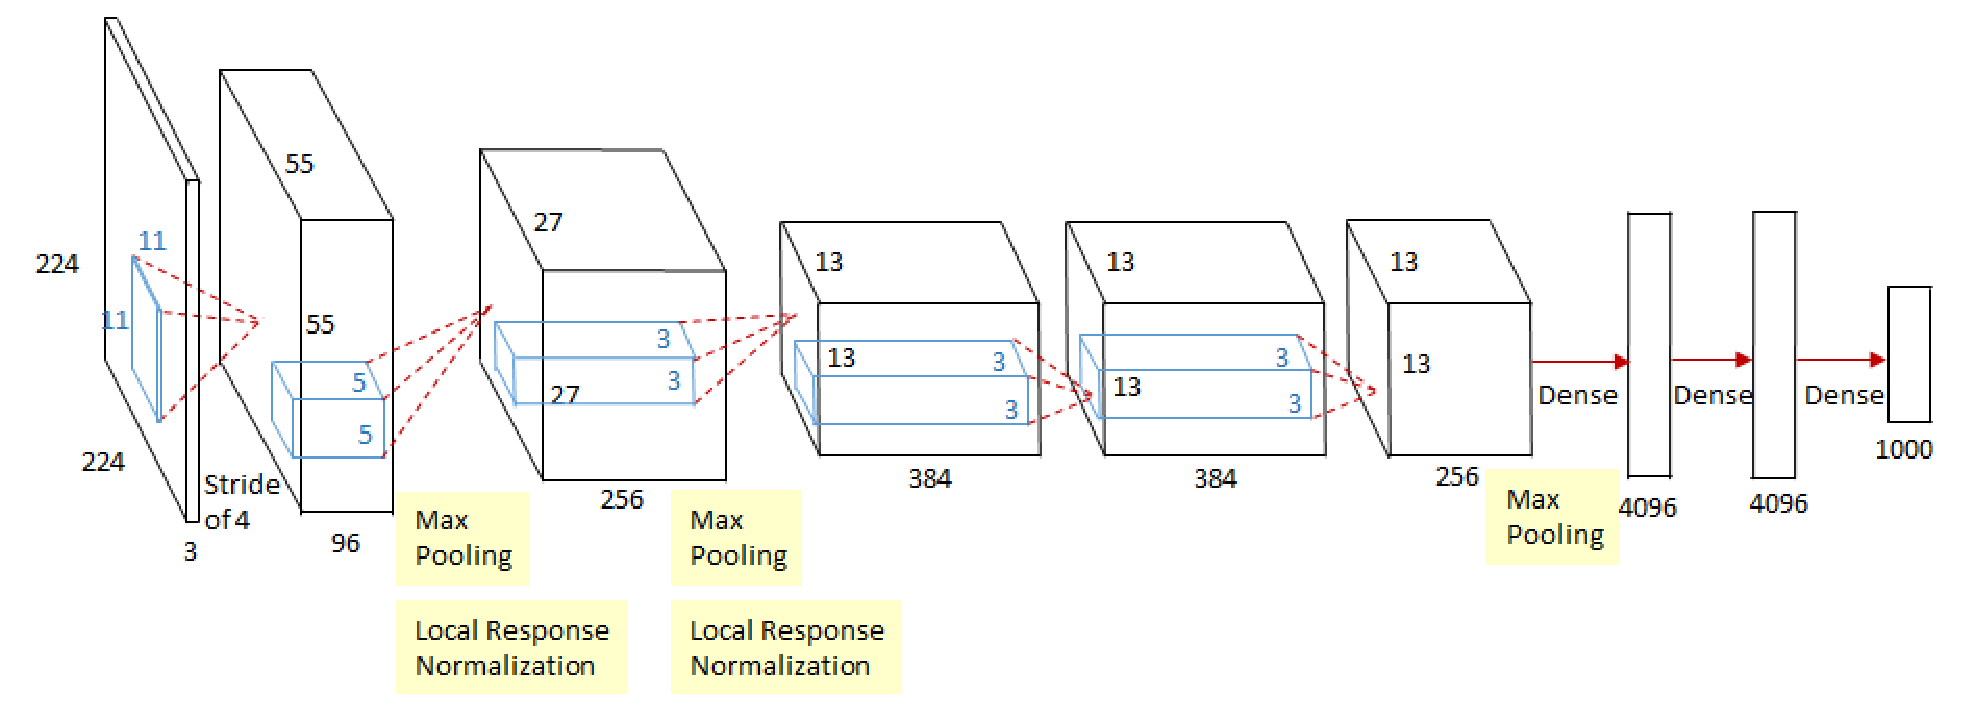
\includegraphics[width=\linewidth]{fig/caffenet.eps}
    \caption{Layer configuration of CaffeNet \cite{reviewalex}}
    \label{fig:caffenet}
\end{figure}

\subsection{Base FPGA implementation}

This section shows the implementation used on the first iteration of the CaffeNet neural network.
Each of the layers were implemented as OpenCL kernels that the compiler transforms into a binary
file that can be used to reprogram the FPGA directly from the Yocto Linux distribution ran
on the ARM Cortex-A9 processor.

\subsubsection{Host code}

The host code is developed using C++, following common \intelOCL examples. The code for this
project is in charge of inserting the training weights file into each of the layers of the
FPGA, as well as resizing the images to fit the 224{x}224{x}3 requirement. The code is capable
of processing only images with .jpeg or .jpg extensions and accepts directories in order to
process a batch of images.

After finishing evaluating each of the images, the code retrieves the values of the output 
matrix in the FPGA and prints the final classification on the screen, including up to the first 
5 possibilities in order to properly evaluate top-1 and top-5 accuracy.

\subsubsection{Convolution layer}

As specified on \cite{suda}, the convolution layer performs a series of 3-dimensional multiply and accumulate (MAC)
operations. These operations can be simplified by using flattening and rearranging of the input features. This way,
the MAC operations end up being simple multiplications that are accumulated and sent to the output buffer.

The general algorithm is as follows:
\begin{enumerate}
    \item Compute the address locations of the input and kernel matrixes
    of the specific work-item identifier.
    \item Load the kernel and input 2-D matrixes into local memory. The input is loaded
    as input[x][y] and the kernel/weights is loaded as kernel[y][x].
    \item Apply the MAC operation as follows: 
    
    output += kernel[y][k]*input[x][k]
    \item Wait until all work-items finish the work.
    \item Save the output to the output buffer using the SDK channels.
\end{enumerate}

These steps must be repeated for every neuron. This process can be optimized using OpenCL
pragma directives to allow for Single Instruction Multiple Data (SIMD) processing. The
parameters that define the convolution layer can be seen in Table \ref{table:convlayer}.
Static parameters are defined for every layer, while dynamic ones are defined per layer
using a JSON description of the network.

The stride and pad are used to determine the index of the input matrix.
Also, each kernel uses a local memory buffer to store the results of each operation.
The buffer size is modified by the SIMD factor, as doing multiple operations at
once requires multiple sections of memory.

\begin{table}[H]
    \begin{center}
        \caption{Parameters used on the convolution layer.}
        \begin{tabular}{lll}
        \hline
        Value                 & Type    & Usage                           \\ \hline
        CHANNEL\_N\_VECTORIZE & Static  & MAC SIMD factor                 \\
        CHANNEL\_N\_WIDTH     & Static  & Neuron SIMD factor              \\
        CONV\_CH\_SIZE\_BUF   & Static  & Local memory buffer             \\
        CONV\_CH\_SIZE\_BUF   & Static  & Local memory buffer             \\
        CONV\_CH\_STRIDE      & Dynamic & Stride to use per layer         \\
        CONV\_CH\_PAD         & Dynamic & Padding to add to input feature \\ \hline
        \end{tabular}
        \label{tab:convlayer}
    \end{center}
\end{table}

\subsubsection{Pooling}

The pooling layers are implemented using overlapping max pooling, following AlexNet's
configuration. This means that the kernel downsample the input by selecting the maximum
value of each input window matrix and the stride used results in overlapping results.

The algorithm is a simple iteration over each of the values of the window and selecting
the maximum. The parameters used in this type of layer are shown in Table \ref{table:poolinglayer}
The SIMD factor determines the size of the local memory to be used.

\begin{table}[H]
    \begin{center}
        \caption{Parameters used on the pooling layer.}
        \begin{tabular}{lll}
        \hline
        Value                 & Type    & Usage                   \\ \hline
        CHANNEL\_N\_WIDTH     & Static  & Neuron SIMD factor      \\
        CONV\_SIZE\_BUF       & Static  & Local memory buffer     \\
        POOL\_CH\_EXTEND\_MAX & Static  & Local memory buffer     \\
        POOL\_EXTEND          & Dynamic & Internal SIMD factor    \\
        POOL\_STRIDE          & Dynamic & Stride to use per layer \\ \hline
        \end{tabular}
        \label{tab:poolinglayer}
    \end{center}
\end{table}

\subsubsection{Normalization}

Local response normalization (LRN) is applied using the formula described in
section \ref{theorylrn}. The algorithm followed to compute normalization for
each kernel is the following:

\begin{enumerate}
    \item For each \textit{input\_feature i}:
    \item For each neuron \textit{j} in feature \textit{i}:
    \item Compute \textit{sum\_of\_squares[j] += input\_feature[i+n/2][j]}
    \item Compute \textit{output\_feature[i][j] = input\_feature[i][j]*pwlf(k+$\alpha$*sum\_of\_squares[j])}
    \item Update \textit{sum\_of\_squares[j] –= input\_feature[i–n/2][j]}
\end{enumerate}

Where \textit{pwlf} is an approximate function with precomputed values. This
function is hard-coded to avoid doing the calculations in the FPGA and returns the value
of the exponential part of the equation in section \ref{theorylrn}. Exponential functions
are hard to implement hardware-wise, a version with approximate values using a dictionary
implemented directly as a ROM section is faster and provides the same functionality.

Table \ref{tab:normalizationlayer} shows the parameters used to configure the execution
of the normalization layer. Just like the other layers, a SIMD factor is used and can be
modified to increase the resource usage of the FPGA being used.

\begin{table}[H]
    \begin{center}
        \caption{Parameters used on the normalization layer.}
        \begin{tabular}{lll}
        \hline
        Value                  & Type    & Usage               \\ \hline
        CHANNEL\_N\_VECTORIZE  & Static  & Neuron SIMD factor  \\
        NORM\_N\_SLICES\_MAX   & Static  & Local memory buffer \\
        NORM\_SIZE\_IN\_MAX\_0 & Static  & Local memory buffer \\
        NORM\_N\_SLICES        & Dynamic & Memory access index \\
        NORM\_N\_SLICES\_MIN   & Static  & Internal SIMD factor \\ \hline
        \end{tabular}
        \label{tab:normalizationlayer}
    \end{center}
\end{table}

Normalization also allows for parallel SIMD operations. Each neuron can do its work
separate from the others and the normalization operation can also be applied in parallel
for each input feature slice. The slices determine how much work can be done per neuron
on each part of the input matrix.

\subsubsection{Fully Connected Layer}

The fully connected layer does the same work as the convolution layer, with the difference
that it is connected to every output from the layer before it. The parameters used are the
same.

\subsubsection{Activation Function}

AlexNet uses Rectified Linear Unit (ReLU) as the activation function. 
It is defined as f(x) = max(0,x) and it is applied after every convolution layer.
It allows to filter out negative values and provides non-linearity between layers. It also
has low computational complexity, as it is easy to implement.

% talk about channels if there is not enough pages

\subsection{Approximate changes}

Any approximate changed done in order to reduce the accuracy but improve the performance
and resource usage is described in the following sections.

\subsubsection{Arbitrary precision}

The fixed-point precision is defined for each layer on the JSON description of the network.
Each number contains an integer and fractional part, but are stored in the same variable.
To determine the bit length and position of the variable, a simple notation is used: 
\textit{[l,p]}, where \textit{l} is the length and \textit{p} is the position of the decimal
point from right to left.

The main objective of using lower precision values for different layers is to reduce the
resources needed in order to execute the network in the FPGA.

As an example, the decimal value 3.25 can be represented using the notation \textit{[5,3]}.
This yields the following binary number:

$$
11_2.010_2
$$

Fixed-point precision can change from the input of one layer to its output. This is achieved
by aligning the precision before applying the specific operation. The limitation is that the
input precision of a layer must match the output precision of the layer before it.m

Aside from manually implementing fixed-point precision, \intelOCL allows for implementation
of compilable arbitrary precision integers. Listing \ref{code:arbitrary} shows a simple
multiplication of two 7-bit integers, the result being saved into a 14-bit integer. The
compiler automatically assigns the desired amount of bits for each variable.

\begin{lstlisting}[language=C++, caption=Arbitrary precision integers, yielding
a 14 bit result, label=code:arbitrary]
// Intel FPGA arbitrary precision integers
uint7_t a2, b2;
uint14_t c2;
c2 = a2 * (uint14_t)b2;
\end{lstlisting}

\subsubsection{Approximate operations}

A CNN spends most of its computational resources on operations within the layers. These operations
can be changed to an approximate version of themselves. Some of the approximations used are:

\begin{itemize}
    \item Approximate MAC: using Adams \cite{adams2019energy} implementation of an energy-efficient
    and approximate MAC unit, gains in resource usage are expected. The execution time changes
    are unknown as Adams did not measure this specific parameter.
    \item Faster pooling operation: pooling operation iterates over the input matrix
    looking for the maximum value on each window. A faster operation can ignore specific
    values or skip loop iterations.
\end{itemize}

\subsubsection{OpenCL compiler optimizations}

OpenCL offers optimizations that promise increases in performance at the cost of accuracy.
This optimizations are set on compile time and are specific to OpenCL, not Intel's implementation
for the FPGA. The main approximations used are:

\begin{itemize}
    \item -fp-relaxed: relaxes the order of arithmetic operations. This is only applied 
    to operations on which the order does not affect the end result.
    \item -fpc: Removes intermediary roundings and conversions when possible, 
    and changes the rounding mode to round towards zero for 
    multiplies and adds.
    \item -cl-mad-enable: changes MAC operations to a mad. This is an approximate version of
    MAC with reduced accuracy.
\end{itemize}

There is no control on where these optimizations are applied, as it is set for the whole
compilation process.

\subsubsection{Memoization}

Memoization is applied mainly on convolution layers with small stride values. This is because
the objective is to approximate the overlapping calculations for each neuron. This is achieved
by skipping every other loop call in the main convolution functionality and using the latest
result as the output for every skipped iteration.

\subsubsection{CaffeNet definition changes}

Some approximations that can be applied to the CNN are changing the configuration of the network
in order to reduce the amount of computation done or approximate its results.

\begin{itemize}
    \item Reduction of filter size: AlexNet uses 11{x}11 filters on the first layer. This size
    can be modified to a lower number in order to reduce the number of operations and the
    resource usage of the network. Another
    possibility is to change to specific constant values some of the iterations in the calculations.
    \item Increasing stride value: similarly to memoization, a bigger stride results in big gains
    on computation speed. This change should not affect the resource usage.
    \item Removal of layers: AlexNet achieves its low error-rate by increasing the number of layers
    in its definition. But a higher error-rate with gains in performance and resource usage is
    possible by reducing the depth of the network. This change can only be applied to the later
    layers, as a propagation from the initial layers would require retraining the network, which
    takes longer than the allocated time for the project.
\end{itemize}

\subsection{Validation and measurements}

The methods used to measure and validate the accuracy gains and losses, as well as the
improvement or degradation on performance and resource usage are described in the following
sections.

\subsubsection{Accuracy}

The original validation set used by AlexNet consists of 120000 images from 1000 classes.
Due to limitation in time, the set used in the project consists of only 4000 images.
Accuracy is measured against top-1 and top-5 classification. Each image has a specific class
assigned to it and the validation process returns a matrix with possibilities
for each class.

A Python 3.5 script is used in order to evaluate the validation results of each compiled
CNN against the expected results. The process is a counting of \textit{hits} (good results) for
the first class (top-1) and counting of \textit{hits} for the first 5 classes (top-5).

The actual error-rate is calculated as follows:

$$
Top1_{error} = \frac{\#images - \#top1_{hits}}{\#images}
$$
$$
Top5_{error} = \frac{\#images - \#top5_{hits}}{\#images}
$$

\subsubsection{Performance}

After the input image is resized and transformed into the input matrix, the start time
is measured and when the process is finished, the end time is measured again. The difference
between both times is used as the execution time of the network.

\subsubsection{Resource usage}

\intelOCL provides HTML reports of the estimated resource usage during and after compilation time.
The report contains information on the usage of the following resources:
\begin{itemize}
    \item Adaptive look-up tables (ALUTs): represent the percentage of
    available logic resources used in compiled designed. Each adaptive logic module (ALM)
    can be used to implement two ALUTs.
    \item Registers (FFs): represent the rest of the logic implementation within the
    FPGA.
    \item Digital signal processing units (DSPs): specialized DSP units used by the FPGA
    on complex operations.
    \item Random access memory (RAMs): local memory available within the FPGA. No external RAM
    is being used for this project, so this percentage represents the actual memory usage
    of the whole network.
\end{itemize}

All of these resources should go down when implementing approximate versions of the CNN.

\section{Results and analysis}

The following sections show all relevant results from applying approximate modifications
to the base CNN implementation. These results are compared to the CPU implementation
in regards to accuracy loss and performance. Resource usage is evaluated against
the first version of the working FPGA implementation.

Table \ref{tab:mainresults} shows the different measurements for every major modification. 
The original AlexNet implementation data is used to compare against the results obtained 
in the project. Discrepancies between the the original AlexNet implementation and the
Python implementation are due to using different validation data sets, as the current
project uses a newer data set obtained from downloading test images from image-net.org.

\begin{table}[H]
    \begin{center}
        \caption{Execution time, error rate and resource usage for different types of kernel and approximate modifications.}
        \resizebox{\textwidth}{!}{
            \begin{tabular}{lllllll}
            \hline
            Implementation                   & Top-1 Error (\%) & Top-5 Error (\%)    & Execution time (ms) & ALUTs (\%) & FFs (\%) & RAMs (\%) \\ \hline
            AlexNet                          & 40.7             & 18.2                & -                   & -          & -        & -         \\
            Python CaffeNet                  & 25.53            & 9.37                & 451                 & -          & -        & -         \\
            Base FPGA (8-bit precision)      & 62.79            & 35.39               & 205                 & 92         & 53       & 11        \\
            Fixed-point 7-bit (all layers)   & 94.94            & 79.88               & 203                 & 81         & 45       & 9         \\
            Approximate pooling              & 70.34            & 46.58               & 198                 & 92         & 53       & 11        \\
            All OpenCL optimizations         & 62.79            & 35.39               & -                   & 107        & 57       & 11        \\
            Memoization (all pooling layers) & 71.45            & 47.00               & 196                 & 92         & 53       & 12        \\ \hline
            \end{tabular}}
            \label{tab:mainresults}
    \end{center}
\end{table}

The results from Table \ref{tab:mainresults} are a summary of the main modifications done
on the CNN implementation. They show modifications done on the extreme cases for every
modification (applying modifications to all/none of the layers). As such, the accuracy
varies a lot from the base implementation. As for performance, the initial performance of
205 ms on the 8-bit implementation is used as the base for any comparison to other
modifications.

\subsubsection{Fixed-point}

Figure \ref{fig:fpaccuracy} and Figure \ref{fig:fpperformance} show the accuracy degradation 
and performance gain after
modifying different layers and with two fixed-point configurations, 8-bit and 7-bit.
8-bit is used on all layers and represents the original version of the FPGA implementation.
This is due to limitations on the DE1-SoC FPGA.

\begin{figure}[H]
    \centering
    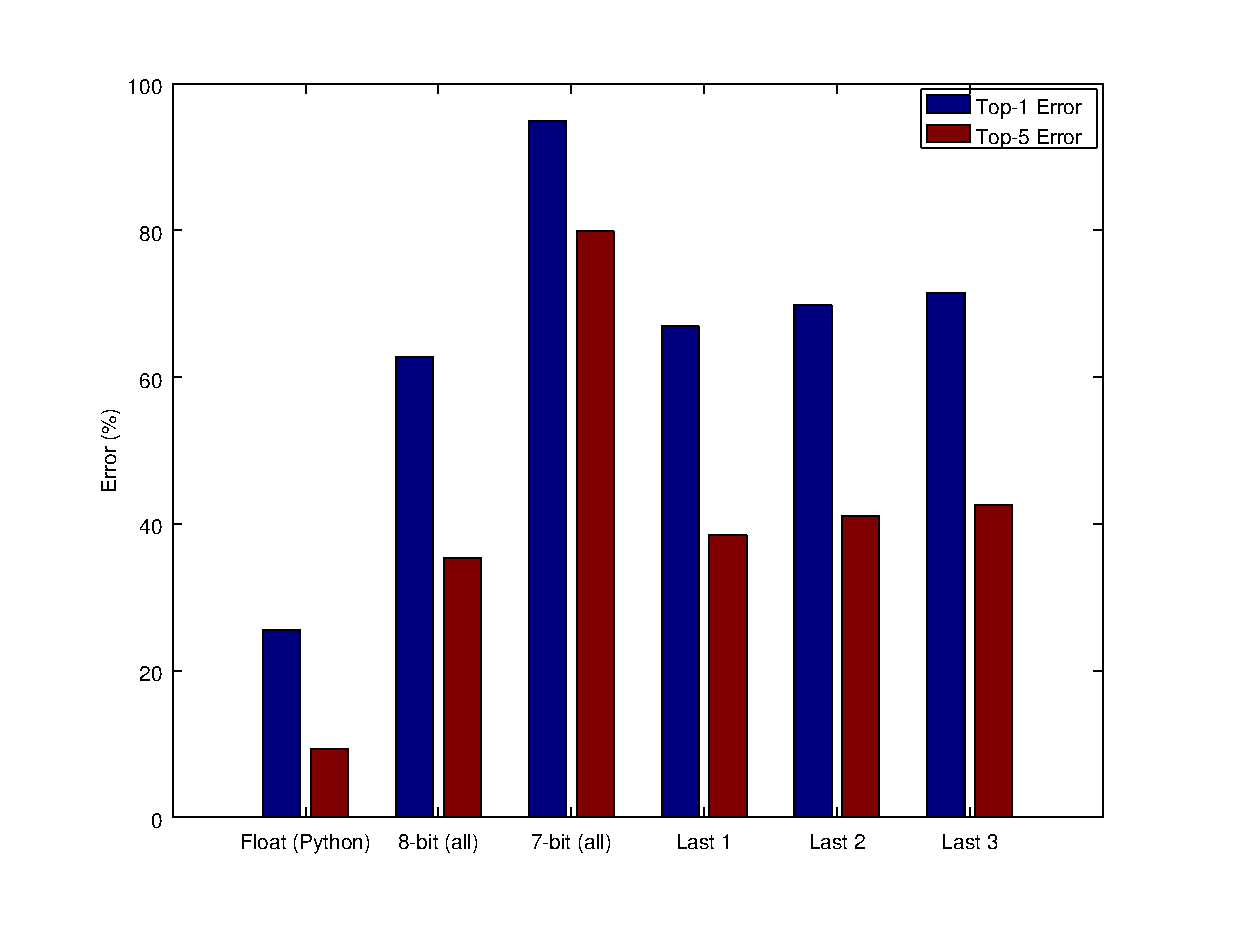
\includegraphics[height=8cm]{fig/fpaccuracy.eps}
    \caption{Error rate results on top-1 and top-5 accuracy for various fixed-point configurations}
    \label{fig:fpaccuracy}
\end{figure}

\begin{figure}[H]
    \centering
    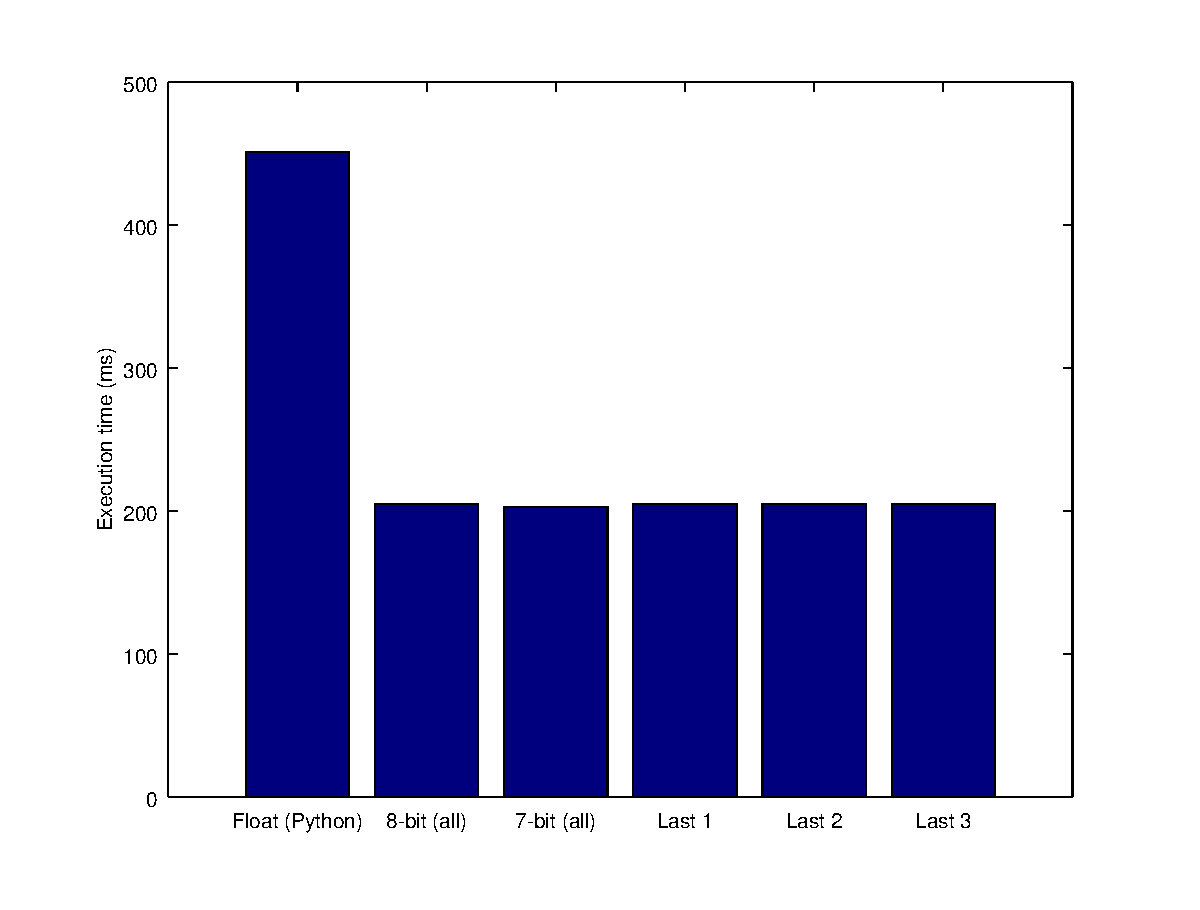
\includegraphics[height=8cm]{fig/fpperformance.eps}
    \caption{Execution time results for various fixed-point configurations}
    \label{fig:fpperformance}
\end{figure}

Making changes to all layers of the CNN greatly degrades the accuracy of the network.
This is because of propagation of the error from the first layers to the later ones.
Because this error is also being approximated, the final result shows a big reduction 
on accuracy. For 7-bit precision on all layers, the loss in accuracy is unacceptable as
the Top-1 error rate falls way above 50\%. But, the loss in accuracy for applying 
this precision on the later layers reflects better results that get close to the 8-bit implementation.

Regarding performance for fixed-point modifications, the changes do not reflect big reductions
in execution time. The main reason is that the number of operations stay the same. The reduction
in resource usage, shown in Table \ref{fig:fpresource}, can be utilized to increase parallelism
of the neuron operations and, in doing so, reduce execution time.

\begin{figure}[H]
    \centering
    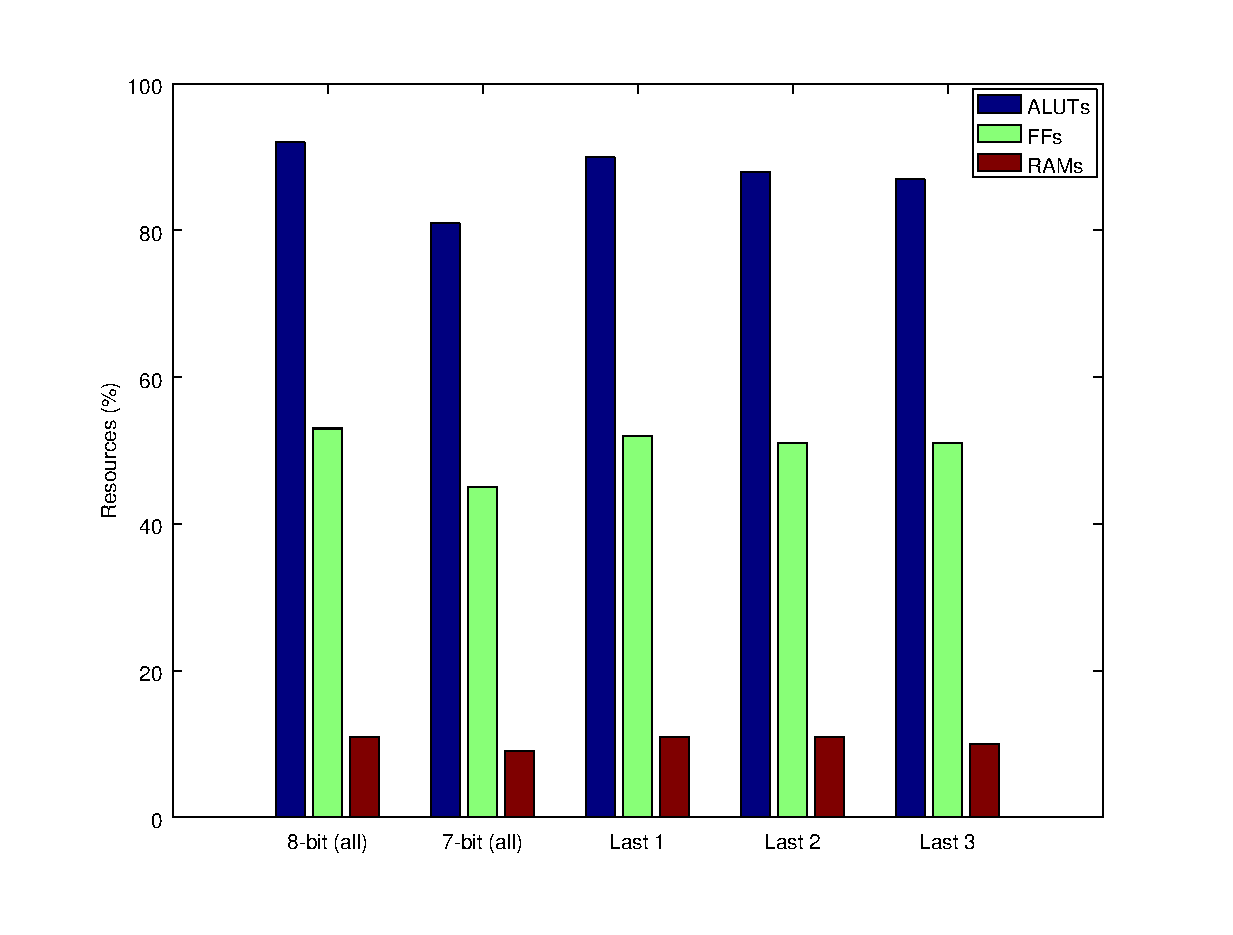
\includegraphics[height=8cm]{fig/fpresource.eps}
    \caption{Resource usage results for various fixed-point configurations}
    \label{fig:fpresource}
\end{figure}

\subsubsection{Approximate operations}

Approximate MAC operations on convolutional/fully-connected layers was tested in combination with
approximate pooling operation. Figure \ref{fig:operationaccuracy} shows the accuracy loss after
applying one of each operation and their combination.
The error rate is increased greatly for the MAC operation. This is because MAC is the most
common operation in the CNN, while pooling is only done on three of the layers.
These operations are applied to the all layers of the same type.

\begin{figure}[H]
    \centering
    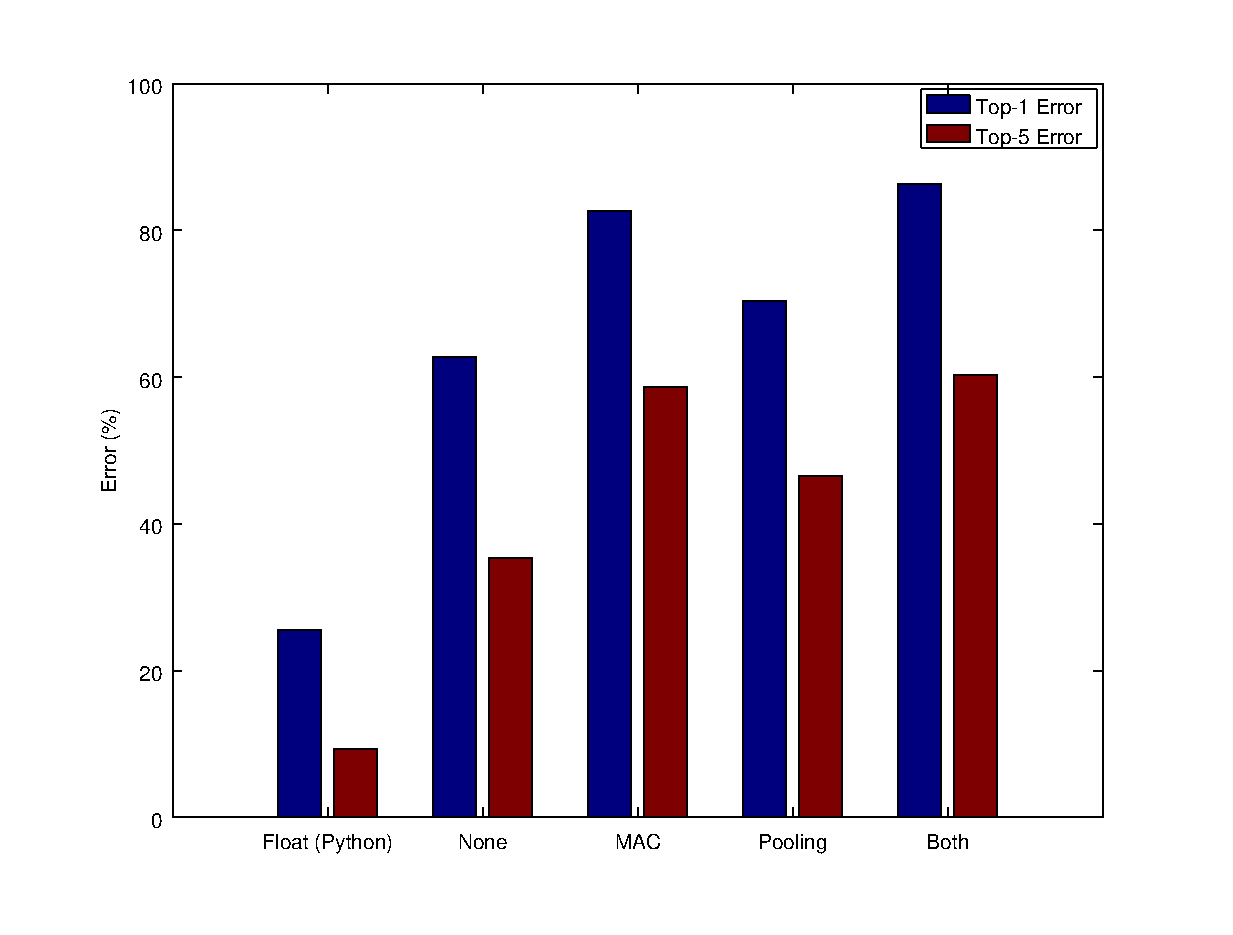
\includegraphics[height=8cm]{fig/operationaccuracy.eps}
    \caption{Error rate results on top-1 and top-5 accuracy for various approximate operation implementations}
    \label{fig:operationaccuracy}
\end{figure}

\begin{figure}[H]
    \centering
    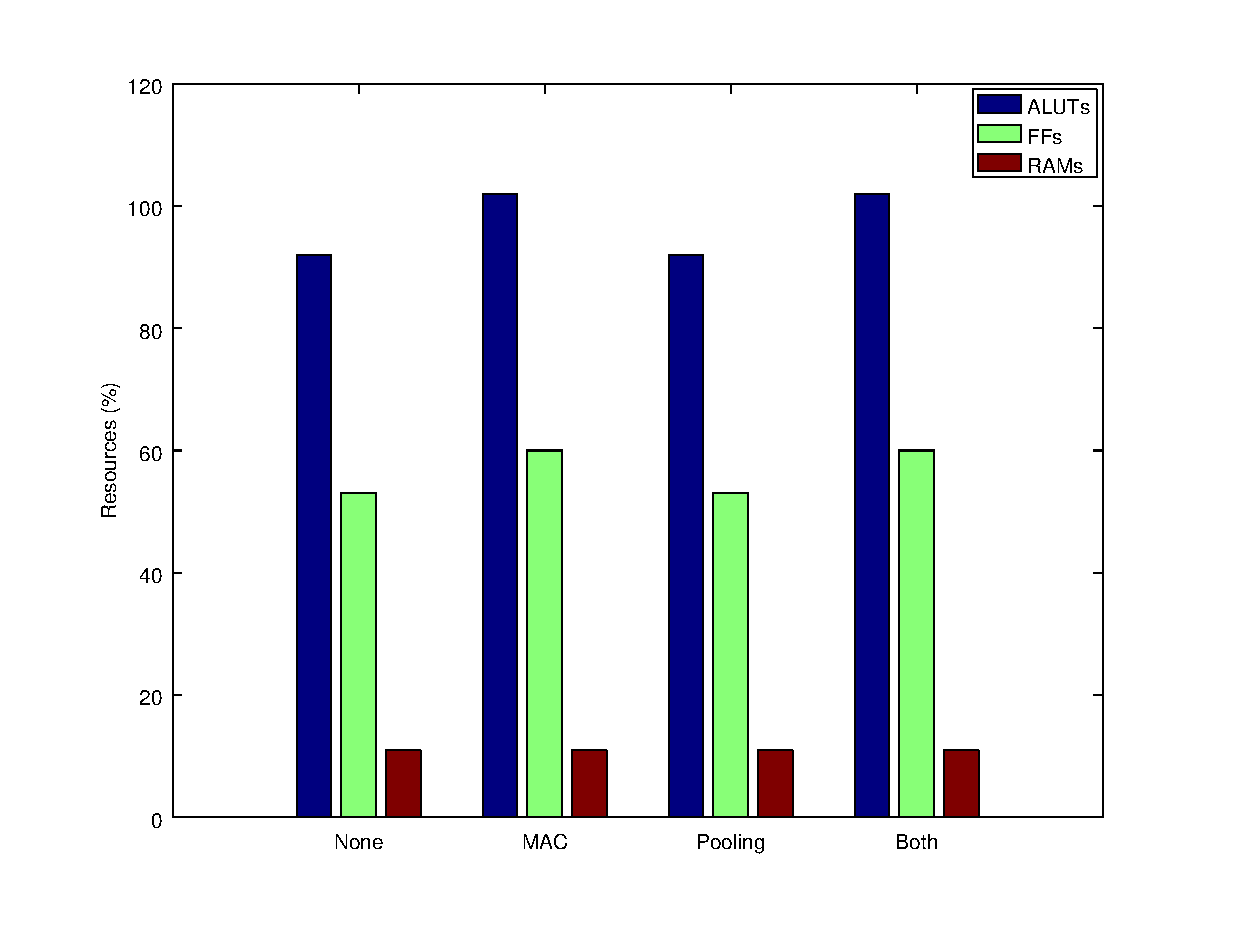
\includegraphics[height=8cm]{fig/operationresource.eps}
    \caption{Resource usage for various approximate operation implementations}
    \label{fig:operationresource}
\end{figure}

On figure \ref{fig:operationresource}, the resource usage for each combination is seen. The resource
usage for the MAC operation exceeds the available resources on the DE1-SoC board because of the way
they had to be implemented on OpenCL, using bit-level shifting to apply approximation. As OpenCL
does not allow for bit manipulation within a variable, the resulting implementation requires more
resources than the regular multiplication. Pooling does not show any changes in resource usage,
as the memory used for iteration skipping on the inner loops is minimal.

Performance on approximate operations was only measured for the approximate
pooling operation. Because the resource usage is above the limits of the DE1-SoC board,
the performance could not be measured. Accuracy was measured using an emulation of the
implementation, which allows resource usages above 100\%. The execution time for
the approximate pooling operation is 198ms, almost 4\% faster than the base implementation.
It could be possible to reduce the parallelism of the pooling operation in order to reduce resource
usage.

\subsubsection{OpenCL optimizations}

OpenCL optimizations did not yield any relevant results in terms of performance or
resource utilization. Using the \textit{-fpc} flag resulted in higher than 100\% resource
usage but no changes in accuracy. The most likely reason for no significant differences
is because most of the implementation already contains most of these optimizations within
the actual code. The OpenCL approximation flags work better on native float variables
and operations with these values.

\subsubsection{Memoization}

Memoization on window shifting was applied only to layers with big filter matrix size and low
stride values (less or equal than 2). As such, it was only applied to the three pooling layers.
It is applied to reduce the number of operations in each layer in half, so it is only storing
values once every two iterations of the main inner loop of the layer.
Table \ref{tab:memoization} shows the results of applying memoization to the first, second and third
pooling layers and combination of these. Resource usage increased on memory usage but the performance
is improved because of it, while accuracy is reduced slightly for every change.

\begin{table}[H]
    \begin{center}
        \caption{Execution time, error rate and resource usage for memoization on different layer combinations.}
        \resizebox{\textwidth}{!}{
            \begin{tabular}{lllllll}
            \hline
            Layers applied                   & Top-1 Error (\%) & Top-5 Error (\%)    & Execution time (ms) & ALUTs (\%) & FFs (\%) & RAMs (\%) \\ \hline
            None (Python)                    & 25.53            & 9.37                & 451                 & -          & -        & -         \\
            None (FPGA)                      & 62.79            & 35.39               & 205                 & 92         & 53       & 11        \\
            1st                              & 67.56            & 42.51               & 200                 & 92         & 53       & 12         \\
            2nd                              & 64.91            & 38.22               & 202                 & 92         & 53       & 11        \\
            3rd                              & 63.83            & 36.88               & 204                 & 92         & 53       & 11        \\
            2nd + 3rd                        & 71.45            & 47.00               & 201                 & 92         & 53       & 12        \\
            1st + 2nd + 3rd                  & 71.45            & 47.00               & 196                 & 92         & 53       & 12        \\ \hline
            \end{tabular}}
            \label{tab:memoization}
    \end{center}
\end{table}

Due to implementing this technique on the pooling layers that provide downsampling, the accuracy
is not affected greatly. Pooling is a good choice for approximation as it provides little changes
to accuracy, but the gains in area or performance are not that significant because of the little
amount of operations in comparison to convolution.

\subsubsection{CaffeNet definition changes}

Most of the changes applied in this section should require a retraining of the network. This is
because of the nature of CNNs, as any change in the layer configuration or parameters requires
new weights data for use in future executions. As such, the results are highly subjective to
changes if retraining is done after applying them. Most of the relevant results are related
to resource usage and performance. Accuracy was not measured for these changes due to
limitations on network retraining time.

Filter size was reduced for the convolutional layers. The results can be seen on Table \ref{tab:filter},
with different filter size on different layers. The performance and memory gains can be significant
for smaller filter matrixes.
Reducing filter size is a change that greatly changes the configuration of the network, but
can be applied with retraining.

\begin{table}[H]
    \begin{center}
        \caption{Execution time and resource usage for different configurations of filter size.}
        \resizebox{\textwidth}{!}{
            \begin{tabular}{llllll}
                \hline
                Layer                          & Filter size & Execution time (ms) & ALUTs (\%) & FFs (\%) & RAMs (\%) \\ \hline
                Base FPGA                      & -           & 205                 & 92         & 53       & 11        \\
                \multirow{2}{*}{Convolution 1} & 10x10       & 198                 & 89         & 50       & 10        \\
                                               & 9x9         & 194                 & 87         & 49       & 9         \\
                \multirow{2}{*}{Convolution 2} & 4x4         & 200                 & 89         & 50       & 10        \\
                                               & 3x3         & 198                 & 88         & 49       & 10        \\
                Convolution 3                  & 2x2         & 201                 & 90         & 51       & 10        \\ \hline
            \end{tabular}}
            \label{tab:filter}
    \end{center}
\end{table}

Changes in stride value were done on the convolution and pooling layers. Table \ref{tab:stride}
shows the changes in performance and resource gain for this change on different combinations of
layers, increasing the value of the stride 2 per layer. Resource usage stays the same due 
to not changing the resources used per operation, but
the performance gain is significant.

\begin{table}[H]
    \begin{center}
        \caption{Execution time and resource usage for different stride values.}
        \resizebox{\textwidth}{!}{
            \begin{tabular}{lllll}
                \hline
                Layer                          & Execution time (ms) & ALUTs (\%) & FFs (\%) & RAMs (\%) \\ \hline
                Base FPGA                      & 205                 & 92         & 53       & 11        \\
                Convolution + Pooling 1        & 199                 & 92         & 53       & 11        \\
                Convolution + Pooling 2        & 198                 & 92         & 53       & 11        \\
                Convolution + Pooling 3        & 199                 & 92         & 53       & 11        \\
                Convolution + Pooling 1,2      & 194                 & 92         & 53       & 11        \\
                Convolution + Pooling 1,2,3    & 189                 & 92         & 53       & 11        \\ \hline
            \end{tabular}}
            \label{tab:stride}
    \end{center}
\end{table}

Finally, removal of layers was only done as experimentation. This is the least recommended change as
it means a complete different configuration as Alex/CaffeNet. The only layers that can
be easily removed were the fifth convolution layer and second fully-connected layer, as the
outputs from the layers before and inputs from the layers after match without any further changes.
Table \ref{tab:layers} shows the results in terms of execution time and resource usage. There is
a big gain on both, but retraining is completely required for accuracy measurements.

\begin{table}[H]
    \begin{center}
        \caption{Execution time, error rate and resource usage on removing layers from the configuration.}
        \resizebox{\textwidth}{!}{
            \begin{tabular}{lllll}
                \hline
                Layers removed                 & Execution time (ms) & ALUTs (\%) & FFs (\%) & RAMs (\%) \\ \hline
                Base FPGA                      & 205                 & 92         & 53       & 11        \\
                Convolution 5                  & 190                 & 84         & 48       & 10         \\
                Fully-connected 2              & 191                 & 86         & 50       & 10        \\
                Convolution + fully-connected  & 176                 & 78         & 45       & 9         \\ \hline
            \end{tabular}}
            \label{tab:layers}
    \end{center}
\end{table}